\subsection{Experimento 1}
\subsubsection{Descripción}

\par Se realizaron dos implementaciones alternativas de Imagen Fantasma.
\par Una, en lugar de multiplicar por 0.9, multiplica por 1 (no hace nada).
\par La otra multiplica por 7/8 (0,875) utilizando operaciones de multiplicación de enteros SIMD y shifts en SIMD. A continuación, el código de la misma:

\begin{codesnippet}
    \begin{verbatim}
movdqu xmm1, [rdi + rax]       ; xmm0 = primeros 4 pixeles a partir de i, j


pmovzxbw xmm0, xmm1            ; xmm0 = [2do pixel | 1er pixel]
psrldq xmm1, 8
pmovzxbw xmm1, xmm1            ; xmm1 = [4to pixel | 3er pixel]


movdqu xmm5, xmm0              
; xmm5 = [ a2 | b2 | g2 | r2 | a1 | b1 | g1 | r1 ]
pmulhw xmm5, xmm9              ; xmm5 = 
[ hi(8*a2) | hi(7*b2) | hi(7*g2) | hi(7*r2) | hi(8*a1) | hi(7*b1) | hi(7*g1) | hi(7*r1) ]
pmullw xmm0, xmm9              ; xmm0 = 
[ low(8*a2) | low(7*b2) | low(7*g2) | low(7*r2) | low(8*a1) | low(7*b1) | low(7*g1) | low(7*r1) ]
movdqa xmm6, xmm0              ; xmm6 = 
[ low(8*a2) | low(7*b2) | low(7*g2) | low(7*r2) | low(8*a1) | low(7*b1) | low(7*g1) | low(7*r1) ]
punpcklwd xmm0, xmm5           ; xmm0 = [ 8*a1 | 7*b1 | 7*g1 | 7*r1 ]
punpckhwd xmm6, xmm5           ; xmm6 = [ 8*a2 | 7*b2 | 7*g2 | 7*r2 ]
psrlw xmm0, 3                  ; xmm0 = [ a1 | 7/8*b1 | 7/8*g1 | 7/8*r1 ]
psrlw xmm6, 3                  ; xmm6 = [ a2 | 7/8*b2 | 7/8*g2 | 7/8*r2 ]
packusdw xmm0, xmm6            ; xmm0 = [ 2do pixel | 1er pixel ]

movdqu xmm5, xmm1              ; xmm5 = [ a4 | b4 | g4 | r4 | a3 | b3 | g3 | r3 ]
pmulhw xmm5, xmm9              ; xmm5 = 
[ hi(8*a4) | hi(7*b4) | hi(7*g4) | hi(7*r4) | hi(8*a3) | hi(7*b3) | hi(7*g3) | hi(7*r3) ]
pmullw xmm1, xmm9              ; xmm1 = 
[ low(8*a4) | low(7*b4) | low(7*g4) | low(7*r4) | low(8*a3) | low(7*b3) | low(7*g3) | low(7*r3) ]
movdqa xmm6, xmm1              ; xmm6 = 
[ low(8*a4) | low(7*b4) | low(7*g4) | low(7*r4) | low(8*a3) | low(7*b3) | low(7*g3) | low(7*r3) ]

punpcklwd xmm1, xmm5           ; xmm1 = [ 8*a3 | 7*b3 | 7*g3 | 7*r3 ]
punpckhwd xmm6, xmm5           ; xmm6 = [ 8*a4 | 7*b4 | 7*g4 | 7*r4 ]
psrlw xmm1, 3                  ; xmm1 = [ a3 | 7/8*b3 | 7/8*g3 | 7/8*r3 ]
psrlw xmm6, 3                  ; xmm6 = [ a4 | 7/8*b4 | 7/8*g4 | 7/8*r4 ]
packusdw xmm1, xmm6            ; xmm1 = [ 4to pixel | 3er pixel ]

packuswb xmm0, xmm1            ; xmm0 = [ 4to pixel | 3er pixel | 2do pixel | 1er pixel ]
	\end{verbatim}
\end{codesnippet}




\subsubsection{Pregunta a responder}
\par ¿Cuánta precisión perdemos en el filtro si reemplazamos las operaciones con floats por operaciones con enteros que aproximen multiplicar por 0.9?
¿Cuánta performance se gana? ¿Vale la pena?


\subsubsection{Hipótesis del grupo}
\par En cuanto a performance, se espera que la implementación que multiplica por 1 sea la más veloz con una diferencia notable y que la otra alternativa
sea la segunda más rápida, dejando última a la implementación original.
Por otro lado, en cuanto a la precisión, observando los factores que usamos en los algoritmos, es evidente que la implementación original será la mejor,
dejando atrás a la segunda alternativa y luego a la primera.


\subsubsection{Análisis de los resultados y conclusiones}
\par Para constrastar nuestra hipotesis realizamos dos mediciones distintas. Una, sobre el error existente al utilizar las dos alternativas propuestas contra la original. Luego 
medimos la performance entre las tres implementaciones. En los siguientes gráficos se pueden apreciar los resultados obtenidos.

\begin{figure*}[h]
    \centering
        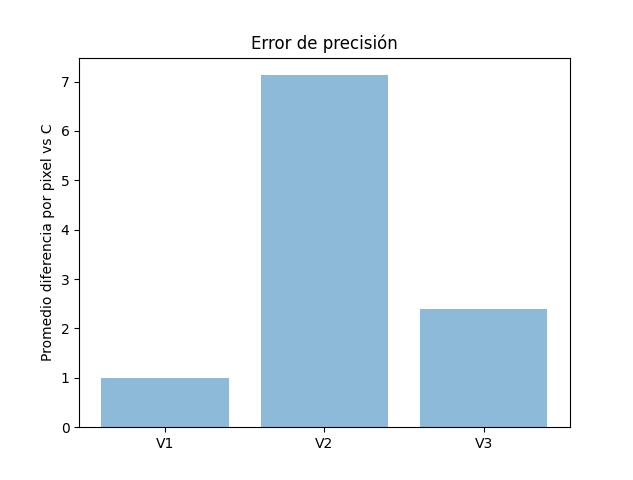
\includegraphics[width=0.5\linewidth]{img/ComparacionErrorExperimentoPato.png}\hfil
        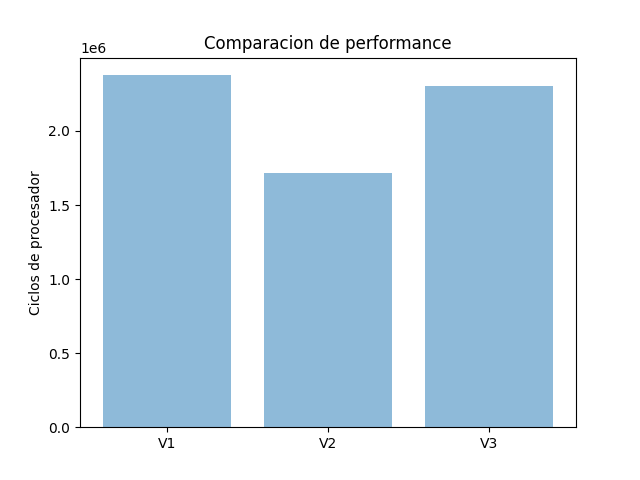
\includegraphics[width=0.5\linewidth]{img/ComparacionPerformanceExperimentoPato.png}\par\medskip
        \caption{Comparación del error entre la implementación original y las dos alternativas}
        \caption{Comparación de performance entre las implementaciones}
\end{figure*}

\par Como se esperaba, la primer alternativa, es sensiblemente más performante que las otras dos. Esto significa que podría ser una opción interesante si se
necesita aplicar el filtro en tiempo real y no se requiere mucha fidelidad. Sin embargo no se notó una diferencia apreciable entre la
implementación original y la segunda alternativa. Esto puede deberse a que contiene múltiples operaciones de pack, unpack, y mov.
\par Por último, la precisión de la segunda alternativa es similar a la de la implementación original, puesto que 7/8 es una aproximación decente de 0.9,
mientras que la primer alternativa es considerablemente peor. Vale la pena notar que la diferencia en las imágenes resultantes de la implementación original y la que tiene peor precisión es altamente
despreciable a simple vista.

\subsection{Experimento 2}
\subsubsection{Descripción}

\par Se corrió la implementación en C del filtro Reforzar Brillo para imágenes del mismo tamaño con los siguientes parámetros: 
\begin{itemize}
	\item un umbral superior de -1, que fuerza en cada iteración a que se entre al primer \texttt{if} y una imagen en negro que provoca siempre el mismo comportamiento en la función saturación
	\item un umbral inferior de 151 y uno superior de 150 que fuerza en cada iteración a que se entre al primer o al segundo \texttt{if}
\end{itemize}
\par La motivación de estos casos era, en primer lugar, predeterminar qué saltos tomará el programa, mientas que en el segundo caso se buscó
maximizar la cantidad de saltos distintos.

\subsubsection{Pregunta a responder}
\par ¿Qué ocurre cuando en el posible flujo del código se toma siempre el mismo camino? ¿Y cuando (a priori) son equiprobables distintos branches? ¿Hay algún mecanismo de predicción de 
saltos que entre en juego? Si lo hay, ¿provoca éste cambios significativos en la performance?

\subsubsection{Hipótesis del grupo}
\par La hipótesis formulada afirma que el mecanismo de predicción de saltos presente en todos los procesadores modernos, sean cuales sean los detalles de su funcionamiento, deberá optimizar 
de alguna manera el caso donde siempre se toma el mismo salto o branch, mientras que en el segundo caso, al ser más impredescible (a menos que se trate de una imagen con todos los píxeles iguales 
o donde todos los píxeles mantienen la misma relación de orden con los umbrales, que no es el caso de este experimento) se espera que haya peor performance del filtro.
Esto se debe a que el procesador tiene más probabilidades de predecir el branch equivocado, y entrarán en juego las penalizaciones por hacer una predicción errónea.

\subsubsection{Análisis de los resultados y conclusiones}
\begin{figure*}[h]
    \centering
        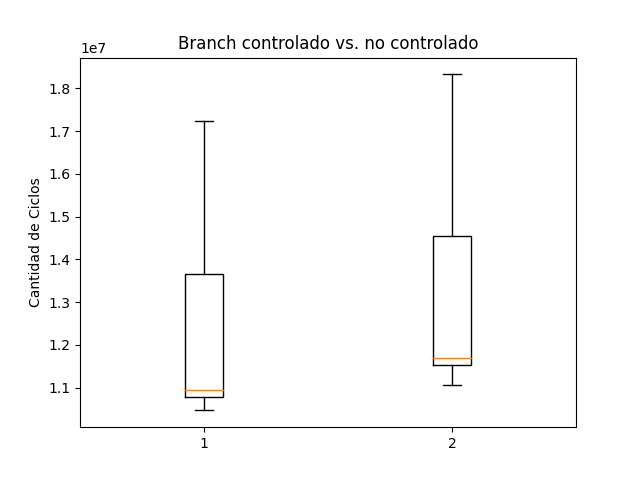
\includegraphics[width=0.5\linewidth]{img/BranchControladoVsNOControlado.jpeg}\hfil
        \caption{Comparación de performance imagen negra vs. imagen normal}
\end{figure*}
\par Se puede observar en la última figura que el rendimiento del primer caso es notablemente mejor que el del segundo. Es evidente que existe una diferencia en el comportamiento del procesador
producto de la imposibilidad de predecir correctamente el camino del segundo caso.